\section{Sprint 2: Creación y gestión de mediciones} %CREAR, EDITAR Y MOSTRAR MEDICIONES


\subsection{Descripción}
En este sprint se llevarán a cabo las interfaces necesarias para que el usuario pueda cargar nuevas mediciones y ver todas sus últimas mediciones ,así teniendo un seguimiento de las mismas con posibilidad de que posteriormente pueda ver su evolución a través de gráficas y tablas.
Para la comunicación de estas interfaces con la API, se desarrollarán los correspondientes adaptadores para los recursos.

Para esto en el backend se deben preparar las clases Measurement, MeasurementType,MeasurementSource,MeasurementUnit con las debidas relaciones con las clase Profile desarrollada en el sprint anterior.
Para cada una de esas clases, se deben preparar interfaces de acceso a los recursos provistos por la API. Y su correspondiente documentación.


\subsection{User Stories relacionados}
La \textbf{Tabla \ref{US-Sprint2}} indicará las características de cada user story para guiarnos en el desarrollo del sprint.

\begin{table}[h]
	%\resizebox{\textwidth}{!}{
    \centering
	\begin{tabular}{|l|p{9cm}|c|}
	\hline
        \multicolumn{1}{|c|}{\textbf{ID}} &
        \multicolumn{1}{|c|}{\textbf{Enunciado de la historia}} &
        \textbf{Prioridad} \\          
    \hline
        US-\ref{resumenInfo} &
        Como paciente quiero obtener un resumen de mi información de salud básica para hacer uso de la misma en caso de una emergencia &Alta
        \\
    \hline 
	    US-\ref{infoSalud} &
        Como paciente quiero cargar mi información personal de salud referido a mediciones (altura, grasa corporal, peso, presión arterial), para que el médico cuente con más y mejor información al momento de realizar el diagnóstico. & Alta
        \\
    \hline
    \end{tabular}
%     }
    \caption{Listado de \textit{User Stories} relacionados.}
    \label{US-Sprint2}
\end{table}

\subsection{Planificación}

\subsubsection{Período de realización}

\begin{itemize}
    \item \textbf{Inicio}: 19 de mayo del 2015.
    \item \textbf{Fin}: 1 de julio del 2015.
\end{itemize}

\subsubsection{Sprint Backlog}

{\scriptsize
	\begin{center} %sidewaystable
		\centering
		%\begin{adjustbox}{max width=\textheight}
		\resizebox{\textwidth}{!}{
			\begin{tabular}{|l|l|l|p{5cm}|l|p{1cm}|}
				\hline
				\textbf{Área a cargo} &
				\textbf{Responsable} &        
				\textbf{Revisor} &        	        
				\textbf{Tarea} &
				\textbf{US} &
				\textbf{Tiempo dedicado} \\
				\hline
				Documentación& Yanina Morales & & Trabajo práctico nº 2 y avance de etapa de diseño &  & 20 horas \\ \hline        
				Documentación& Iván Terreno & & Trabajo práctico nº2 y avance de etapa de diseño  &  & 20 horas \\ \hline        
				Documentación& Michael Manganiello& & Trabajo práctico nº 2 y avance de etapa de diseño  &  & 20 horas \\ \hline        
				Documentación& Franco Canizo & & Trabajo práctico nº 2 y avance de etapa de diseño  &  & 20 horas \\ \hline         
				Front-end & Michael Manganiello& -- & Despliegue de la aplicación en Heroku  & US-\ref{resumenInfo} \& US-\ref{infoSalud}& 4 horas  \\ \hline     
				Capacitación & Yanina Morales& & Capacitación en utilización de Angular de manera desacoplada & US-\ref{infoSalud} & 12 horas \\ \hline        
				Capacitación & Iván Terreno& & Capacitación en utilización de Angular de manera desacoplada& US-\ref{infoSalud} & 12 horas\\ \hline                
				Front-end& Iván Terreno & Michael Manganiello & Generación de controladores para consumir Json de la Api relacionados a la API & US-\ref{resumenInfo} \& US-\ref{infoSalud}& 8 horas  \\ \hline
				Front-end & Yanina Morales& Michael Manganiello & Creación de página de formulario de carga de mediciones& US-\ref{infoSalud} & 4 horas \\ \hline
				Front-end & Iván Terreno  & Michael Manganiello & Creación de página de formulario de carga de perfil& US-\ref{infoSalud} & 4 horas \\ \hline
				Front-end & Iván Terreno  & Michael Manganiello & Realización de pruebas& & 8 horas \\ \hline        
				Front-end & Yanina Morales  & Iván Terreno  & Realización de pruebas & & 12 horas \\ \hline         
				
				Back-end & Michael Manganiello & Franco Canizo & Creación de modulo de mediciones&US-\ref{resumenInfo} \& US-\ref{infoSalud} & 8 horas \\ \hline
				Back-end & Michael Manganiello & Iván Terreno & Exposición de métodos como servicios de API 	& US-\ref{resumenInfo} \& US-\ref{infoSalud} & 8 horas \\ \hline
				Back-end & Franco Canizo & Michael Manganiello   & Adaptación de salida de métodos a formato Json&US-\ref{resumenInfo} \& US-\ref{infoSalud} & 8 horas \\ \hline
				Back-end & Franco Canizo & Michael Manganiello  & Carga de valores a la base de datos, relacionados a la API&US-\ref{resumenInfo} \& US-\ref{infoSalud} & 8 horas \\ \hline
			\end{tabular}
		}
		%\end{adjustbox}
	\end{center}
}

\subsubsection{Actividades de integración}

\begin{figure}[h]
  \centering
  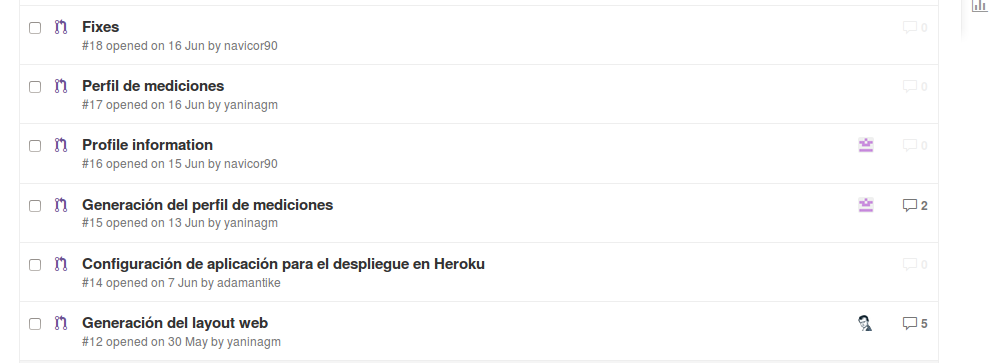
\includegraphics[width=.8\textwidth]{img/2-PR}
  \caption{Pull requests realizados por el front-end.}
  \label{2-PR}
\end{figure}
\begin{figure}[h]
  \centering
  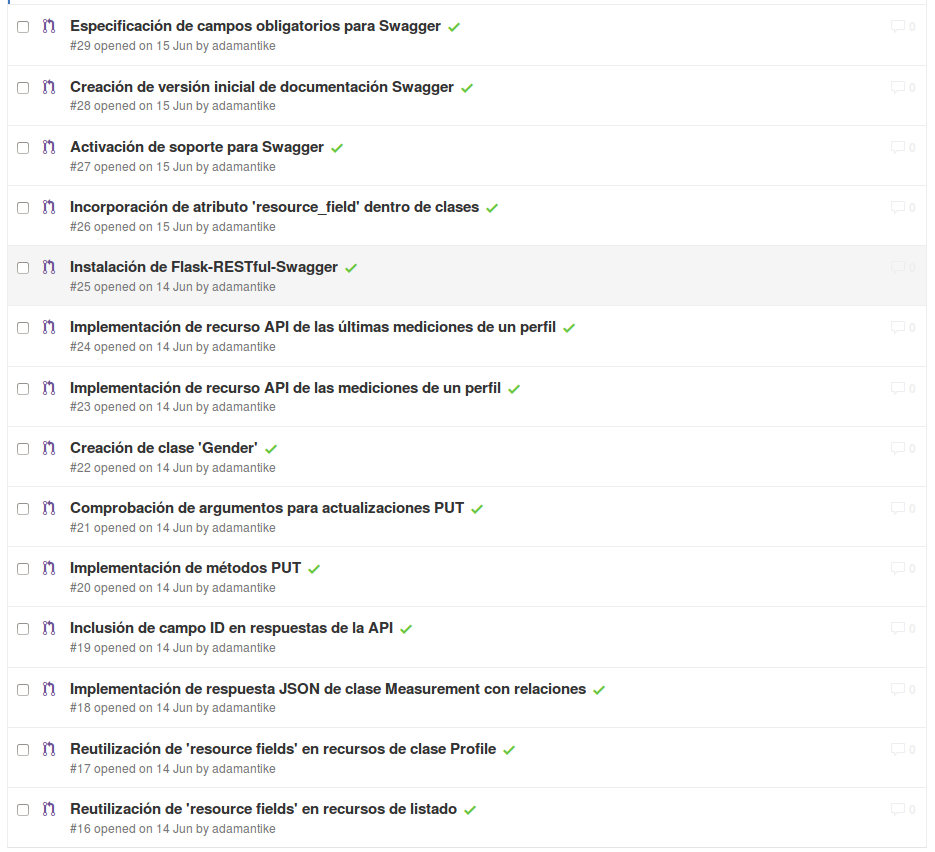
\includegraphics[width=.8\textwidth]{img/2-PR_back2}
  \caption{Pull requests realizados por el back-end, primera parte.}
  \label{2-PR_back2}
\end{figure}
\begin{figure}[h]
  \centering
  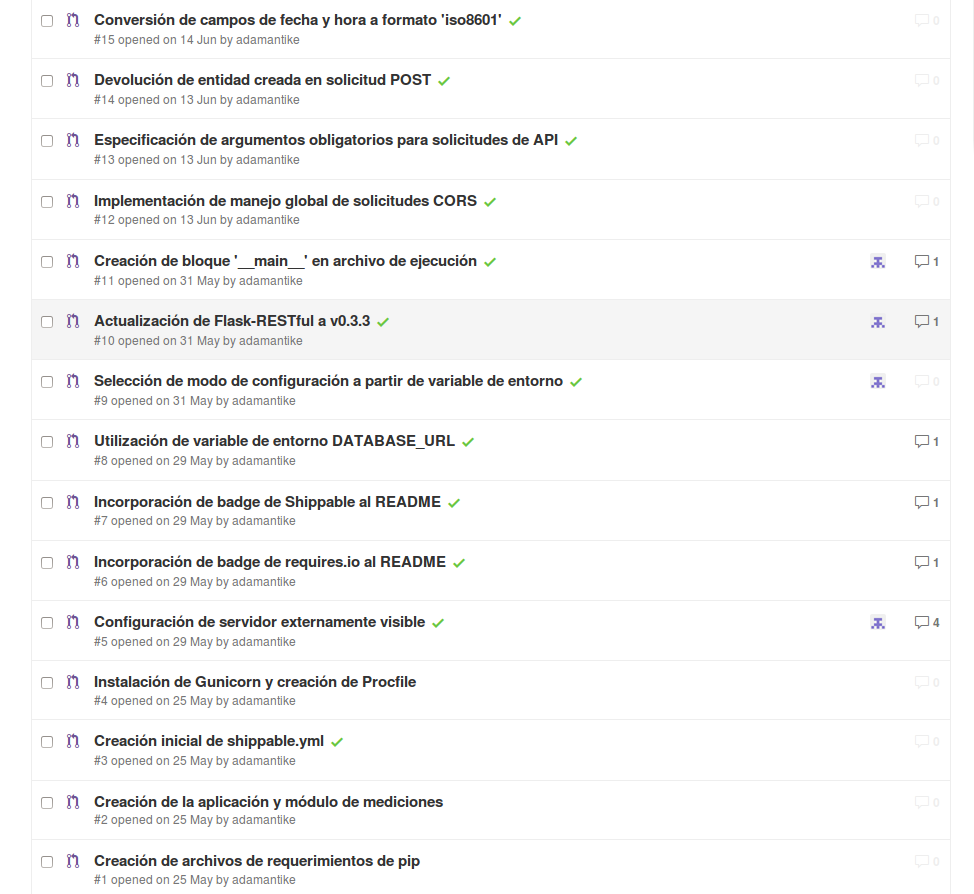
\includegraphics[width=.8\textwidth]{img/2-PR_Back}
  \caption{Pull requests realizados por el back-end, segunda parte.}
  \label{2-PR_Back}
\end{figure}

\clearpage
    
	


\begin{comment}
\subsection{Fase de Análisis}

En esta fase comenzaremos definiendo el Sprint backlog y describiendo en detalle cada una de las tareas que la componen, además se realizará un diagrama de clases iniciales (\textbf{Figura \ref{modelo_datos}}) que nos permitirá guiarnos durante el avance del sprint de ese modo obtener un sistema consistente. 
\end{comment}


\subsection{Modelo de datos}
El Diagrama propio de este sprint se puede ver en la \textbf{Figura \ref{sp2_modelo_especifico}}, allí se indican exactamente las clases que se usarán en este sprint y que serán detalladas con detenimiento en el presente documento. Se recuerda que se ha realizado un Diagrama de clases tentativo que se puede ver en la \textbf{Figura \ref{2-modelo_datos_general}}, dicho diagrama  será utilizado como base para este sprint y posee un alcance limitado el cual se irá modificando a medida que se profundice en los temas.



\begin{figure}[h]
  \centering
  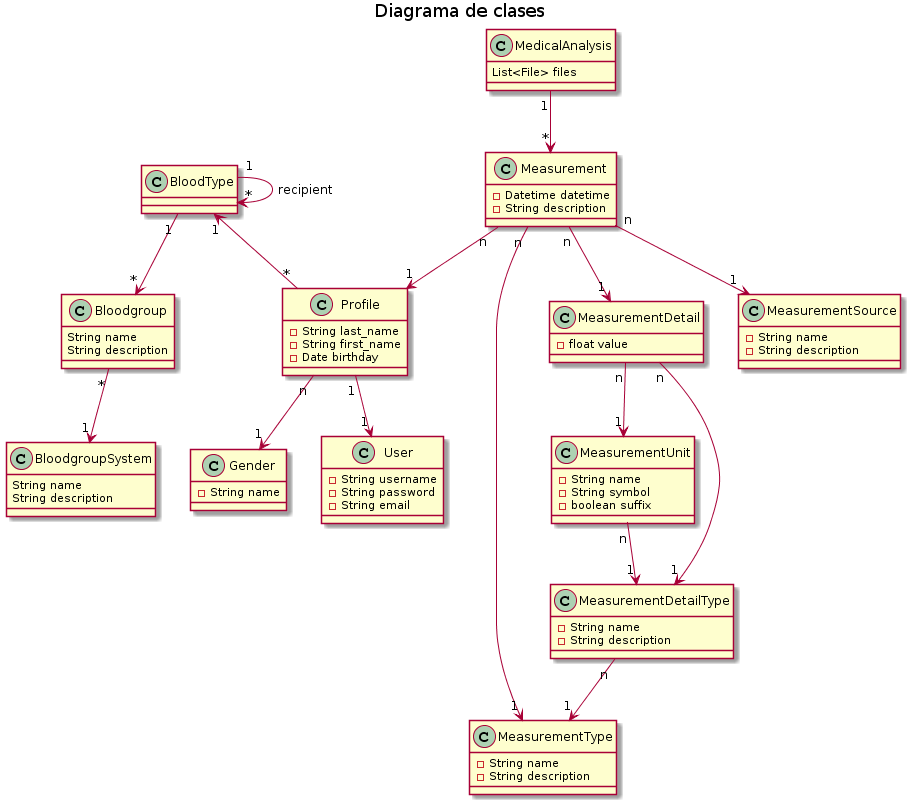
\includegraphics[width=.8\textwidth]{img/2-DC_especifico}
  \caption{Modelo de datos}
  \label{sp2_modelo_especifico}
\end{figure}
\clearpage

\subsection{Descripción de las Clases}

\subsubsection{Clase Measurement} 
Dicha clase se refiere a las medición realizada por el usuario en un momento específico. 

\textbf{Descripción de los atributos}
	\begin{itemize}
		\item \textbf{id:} Identificador único de la medición (tipo int).
        \item \textbf{datetime:} Fecha y hora de la medición (tipo datetime).
        \item \textbf{value:} Valor de la medición (tipo float).
        \item \textbf{profile\_id:} Identificador único del perfil asociado (tipo int).
        \item \textbf{measurement\_source\_id:}Identificador único de la fuente de medición asociada (tipo int).
        \item \textbf{measurement\_type\_id:}Identificador único del tipo de medición asociado (tipo int).
        \item \textbf{measurement\_unit\_id:}Identificador único de la unidad de medición asociada (tipo int).
        
	\end{itemize}
    
\textbf{Dirección del recurso:}
\begin{lstlisting}[language=json,firstnumber=1]
<BASE URL>/measurements/{:id}
\end{lstlisting}

\textbf{Json generado por la API}    
\begin{lstlisting}[language=json,firstnumber=1]
{
    "resource": 
{
    "measurement_unit": 
{
    "symbol": "Kg",
    "suffix": true,
    "name": "Kilogramo",
    "id": 1
},
"measurement_source": 
{
    "name": "Manual",
    "description": null,
    "id": 1
},
"value": 50,
"measurement_type": 
{
    "name": "Peso",
    "description": "Peso corporal de la persona.",
    "id": 1
},
"id": 1,
"profile": 
{
    "birthday": "1990-10-26",
    "last_name": "Terreno",
    "first_name": "Milton",
    "gender": 
            {
                "name": "Masculino",
                "description": null,
                "id": 1
            },
            "id": 1
        },
        "datetime": "2015-06-15T02:29:54"
    }
}
\end{lstlisting}
\subsubsection{Clase MeasurementType}
Esta clase nos permitirá  nomenclar  los tipos de medidas, hasta el momento hemos contemplado: peso, dimensión corporal (Ej:altura) y glucosa. Existen ciertas medidas que contemplan dos valores, estas serán agregadas en un sprint futuro.

\textbf{Descripción de los atributos}
    \begin{itemize}
			\item \textbf{name: }	Nombre del tipo de medición(tipo string).
            \item \textbf{description:} Descripción del tipo de medición (tipo string).
    \end{itemize}

\textbf{Dirección del recurso:}
\begin{lstlisting}[language=json,firstnumber=1]
<BASE URL>/measurement_types/{id}
\end{lstlisting}

\textbf{Json generado por la API} 
\begin{lstlisting}[language=json,firstnumber=1]
{
    "resource": 
    {
        "name": "Peso",
        "description": "Peso corporal de la persona.",
        "id": 1
    }
}
\end{lstlisting}

\subsubsection{Clase MeasurementUnit}
Esta clase nos permitirá  nomenclar  las unidades de medición disponible para que el usuario pueda seleccionarlas cuando realice la medición, hasta el momento hemos contemplado: Kilogramo, gramo, miligramos, metro, centímetro y milímetro.

    \textbf{Descripción de los atributos}
        \begin{itemize}
            \item \textbf{id:	}	Identificador único de la unidad de medición(tipo int).
            \item \textbf{name :	}	Nombre de la unidad de medición ( tipo string).
            \item \textbf{symbol :}		Símbolo de la unidad de medición (tipo string).
            \item \textbf{suffix :}	Variable booleana que indica si el símbolo de la unidad de medición es un sufijo (verdadero) o un prefijo (falso) del valor de la medición (tipo boolean).
        \end{itemize}

    \textbf{Dirección del recurso}
        \begin{lstlisting}[language=json,firstnumber=1]
        <BASE URL>/measurement_units/{id}
        \end{lstlisting}

    \textbf{Json generado por la API} 
        \begin{lstlisting}[language=json,firstnumber=1]
        {
            "resource": 
            {
                "symbol": "Kg",
                "suffix": true,
                "name": "Kilogramo",
                "id": 1
            }
        }
        \end{lstlisting}

\subsubsection{Clase MeasurementSource}
Esta clase nos permitirá nomenclar los tipos de fuentes posibles como pueden ser manual, dispositivo móvil, sistema de salud y dispositivo de salud.
    
	\textbf{Descripción de los atributos}
        \begin{itemize}
            \item \textbf{name 	:}	Nombre de la fuente de medición (tipo string).
            \item \textbf{description 	:}	Descripción de la fuente de medición (tipo String).
        \end{itemize}
    \textbf{Dirección del recurso}
    \begin{lstlisting}[language=json,firstnumber=1]
    <BASE URL>/measurement_sources/{:id}
    \end{lstlisting}

    \textbf{Json generado por la API} 
    \begin{lstlisting}[language=json,firstnumber=1]
{
    "resource": 
    {
        "name": "Manual",
        "description": null,
        "id": 1
    }
}
    \end{lstlisting}
    
\subsection{Modelo funcional} %Diagrama de clases
Se describirán las funciones usando como marco de apoyo el sprint Backlog, además se armará el diagrama de casos de uso del presente Sprint \textbf{[Figura \ref{2-caso_de_uso}]} que irá creciendo  medida se vaya avanzando en el proyecto.
    \begin{figure}[h]
        \centering
        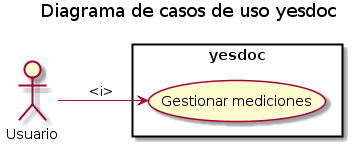
\includegraphics[width=0.5\textwidth]{img/2-caso_de_uso}
        \caption{formulario de edición de perfil}
		\label{2-caso_de_uso}
    \end{figure}

    
\subsubsection{Creación de página de mediciones}
En esta tarea  se generará la pantalla, \textbf{Figura \ref{perfil_medicion}} donde se muestran las mediciones del usuario, como lo son:
      \begin{itemize}
	      \item Altura
          \item Peso
          \item Grasa Corporal
          \item Presión Arterial
      \end{itemize}
      Al igual que en la creación del perfil se dará la posibilidad de acceder a la edición de su perfil desde esta misma página.
      
Para mostrarlas mediciones del usuario es necesario acceder al recurso \texttt{/profiles/\{profile\_id\}/measurements/latest} de la API a través de un método \textbf{GET}


      \textbf{Especificaciones del recursos \texttt{/measurements}}

    \begin{lstlisting}[language=json,firstnumber=1]
          MeasurementFields {
	measurement_source (MeasurementSourceFields, optional),
      profile (ProfileFields),
      datetime (date-time),
      value (number),
      measurement_unit (MeasurementUnitFields),
      id (integer),
      measurement_type (MeasurementTypeFields)
      }
      MeasurementSourceFields {
      description (string, optional),
      id (integer),
      name (string)
      }
      ProfileFields {
      first_name (string),
      last_name (string),
      id (integer),
      gender (GenderFields, optional),
      birthday (date-time, optional)
      }
      GenderFields {
      description (string, optional),
      id (integer),
      name (string)
      }
      MeasurementUnitFields {
      id (integer),
      symbol (string),
      suffix (boolean, optional),
      name (string)
      }
      MeasurementTypeFields {
      description (string, optional),
      id (integer),
      name (string)
      } 
    \end{lstlisting}

    En el perfil de usuario se mostrarán de cada tipo de medición que ha realizado el usuario la última de cada una, indicando el nombre, el valor, el símbolo, la fecha y hora y el método con el que ha sido realizada la medición. Además para cada una de las mediciones se mostrarán dos iconos que corresponden a la edición y a la compartición de las mediciones, este último será implementado en un sprint futuro.

    \begin{figure}[h]
        \centering
        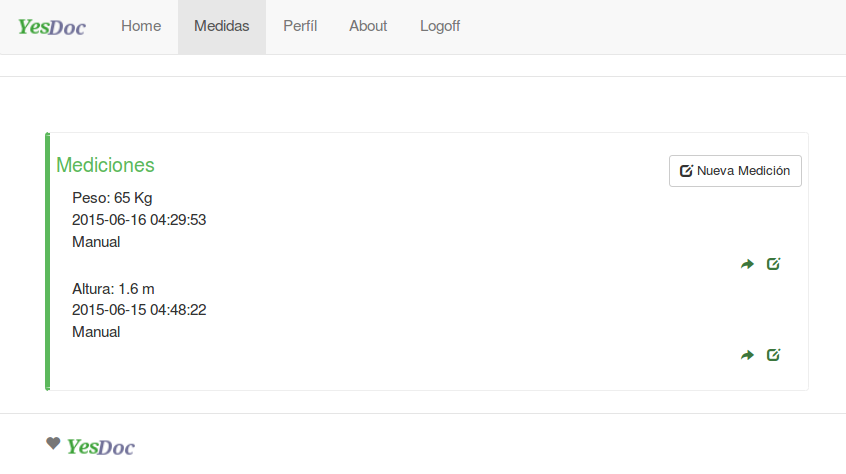
\includegraphics[width=1\textwidth]{img/2-perfil_medicion}
        \caption{Perfil de mediciones}
		\label{perfil_medicion}
    \end{figure}
    
\subsubsection{Creación de página de formulario de carga de mediciones}
Se generará el formulario necesario, que se muestra en la \textbf{Figura \ref{nueva_medicion}} para que el usuario pueda cargar las mediciones antes nombrados, para ello es necesario acceder al recurso \texttt{/measurements} de la API a través de un método \textbf{POST}

      \begin{lstlisting}[language=json,firstnumber=1]
         MeasurementFields {
        measurement_source (MeasurementSourceFields, optional),
        profile (ProfileFields),
        datetime (date-time),
        value (number),
        measurement_unit (MeasurementUnitFields),
        id (integer),
        measurement_type (MeasurementTypeFields)
        }
        MeasurementSourceFields {
        description (string, optional),
        id (integer),
        name (string)
        }
        ProfileFields {
        first_name (string),
        last_name (string),
        id (integer),
        gender (GenderFields, optional),
        birthday (date-time, optional)
        }
        GenderFields {
        description (string, optional),
        id (integer),
        name (string)
        }
        MeasurementUnitFields {
        id (integer),
        symbol (string),
        suffix (boolean, optional),
        name (string)
        }
        MeasurementTypeFields {
        description (string, optional),
        id (integer),
        name (string)
        } 
    \end{lstlisting}
    
Desde el perfil de mediciones se presentará un icono que representa a la creación de un elemento para que el usuario pueda seleccionarlo. Esta acción llevara al usuario al formulario de creación de mediciones, donde los campos estarán vacíos, para que el usuario los cargue con los valores correspondientes. Una vez terminada la carga, se mostrará un mensaje avisando al usuario que se ha realizado con éxito y luego lo direccionará al perfil de mediciones.
    
    \begin{figure}[h]
        \centering
        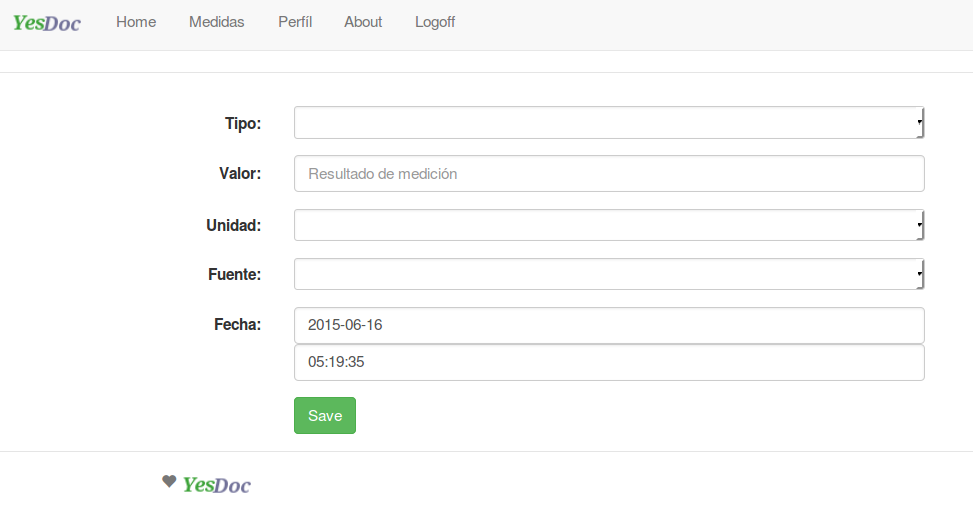
\includegraphics[width=1\textwidth]{img/2-nueva_medicion}
        \caption{Formulario de nueva medición}
		\label{nueva_medicion}
    \end{figure}
\subsubsection{Creación de página de formulario de edición de mediciones}
Se generará el formulario necesario, que se muestra en la \textbf{Figura \ref{editar_medicion}} para que el usuario pueda editar una medición previamente seleccionada, para ello es necesario acceder al recurso \texttt{/measurements/\{:id\}} a través del método \textbf{PUT} enviando por URL el id correspondiente a dicha medición. 

Desde el perfil de mediciones se presentará un icono que representa a la edición de un elemento para que el usuario pueda seleccionarlo. Esta acción llevara al usuario al formulario de edición de mediciones, donde los campos estarán cargados con los valores antiguos, de este modo el usuario modifica lo que desea y no tiene que cargar todo nuevamente. Una vez terminada la edición se direccionará al perfil de mediciones.

	\begin{figure}[h]
        \centering
        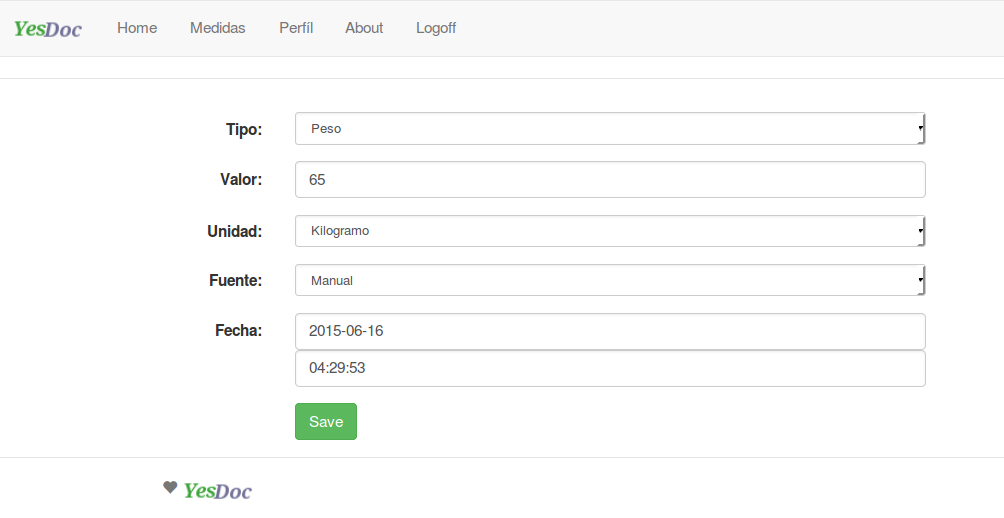
\includegraphics[width=1\textwidth]{img/2-editar_medicion}
        \caption{Formulario de edición de medición}
		\label{editar_medicion}
    \end{figure}
    
%%%%%%%%%%%%%%%%%%%%%% COMPLETAR!!! %%%%%%%%%%%%%%%%%%%%%%%%%%%%
\begin{comment}


\subsubsection{Creación de aplicación  }
\subsubsection{Creación de modulo de mediciones}
\subsubsection{Exposición de métodos como servicios de API}
\subsubsection{Adaptación de salida de métodos a formato Json}
\subsubsection{Creación de base de datos inicial}
\end{comment}

\subsection {Salidas del Sistema - Incrementos}

Luego de finalizado este user story se obtendrán 4 pantallas que se detallarán a continuación:
\begin{enumerate}
    \item \textbf{Presentación de las últimas mediciones}  \textbf{[Figura  \ref{perfil_medicion}]} con posibilidad de edición de cada una de las mediciones. Los datos posible  a presentar son altura, peso, grasa corporal y glucosa. 
    
    La interfaz mostrará el valor de la medición, la fecha y hora en que fue realizada y la fuente que se utilizó para dicha medición.
	\item \textbf{Carga de mediciones}: \textbf{[Figura \ref{nueva_medicion}]} Se le permitirá cargar mediciones que realice en algún momento del día como son peso, altura, grasa corporal y glucosa. Deberá indicar la fuente, tipo, unidad y fecha de la medición
    \item \textbf{Edición de mediciones:}  \textbf{[Figura \ref{editar_medicion}]} Se le permitirá seleccionar una medición del perfil de mediciones para sel modificada.

\end{enumerate}

    




\subsection{Criterios de aceptación}

\begin{center}
\begin{longtable}{|p{0.5cm}|p{4cm}|p{4cm}|p{4.5cm}|}
\hline \hline \rowcolor[gray]{0.9}
	\multicolumn{4}{||c|}{\textbf{Criterio de aceptación}} \\
    \hline  \rowcolor[gray]{0.9}
        \textbf{Id} &
        \textbf{Contexto} &
        \textbf{Evento}&
        \textbf{Resultado} \\
    \hline
1&En caso de que exista una persona sin mediciones & cuando este desee observar sus mediciones  & El sistema no mostrará nada \\ \hline
 
2& Cuando el usuario registrado ingresa dos mediciones del mismo tipo  & y luego quiera consultarlas & El sistema solo le mostrará la ultima medición, del mismo tipo, realizada\\ \hline

3& Cuando el usuario seleccione una medición & y luego quiera editarla & El sistema le permitirá la correspondiente edición\\ \hline

4& Si el usuario existe y no está logueado & y quiera ingresar a ver sus mediciones. & El sistema no le permitirá ingresar\\ \hline
  \end{longtable}
\end{center}


\subsection{Casos de Prueba}


	\begin{table}
	\centering
	\begin{tabular}{|m{4cm}|m{9cm}|}
    	\rowcolor[gray]{0.9}
        \hline 
	    \textbf{Caso de prueba} & \textbf{Consultar mediciones (sin medidas precargadas)}\\  \hline
	    \textbf{Descripción del escenario}& Nombre: Marita; Apellido Martinez; fecha de Nacimiento:20-08-1989; id:3  \\ \hline
	    \textbf{Criterio de aceptación}&  \textbf{En caso de que exista una persona sin mediciones cargadas, si el usuario desea verlas el sistema no debería mostrar ninguna medición.} \\ \hline
        \textbf{Datos de entrada}&  consultar mediciones\\ \hline
        \textbf{Condiciones de  prueba}& Se necesita que esté previamente cargado el usuario ``Marita Martinez'' y no tenga datos más allá de su nombre y apellido en el perfil \\ \hline
	    \end{tabular}
        \caption{Caso de prueba para criterio de aceptación 1}
    	\end{table}
  
{\scriptsize
	\begin{table}[h]
    \centering
	\begin{longtable}{|p{5cm}|p{5cm}|p{5cm}|}
	    \hline \hline \rowcolor[gray]{0.9}
        \multicolumn{3}{||l|}{\textbf{Procedimiento de Prueba - ``Consultar mediciones''}} \\
        \hline \rowcolor[gray]{0.9}
		    \textbf{Actor} & 
	        \textbf{Sistema}& 
        	\textbf{Resultado esperado} \\  
        \hline
	    El usuario ingresa al sistema con su id nº3	& &\\ \hline
        		& El sistema valida con los perfiles de la API si el Id:3 del usuario existe& Se presenta por pantalla el perfil del usuario con sus datos  \\ \hline        
	    El usuario selecciona la pestaña mediciones y realiza la consulta& &\\ \hline
      	&El sistema valida que las cookies estén activas&\\ \hline
   		&El sistema solicita a la API las mediciones del perfil con id:3&El sistema no muestra ninguna medida cargada \\ \hline 
	    \end{longtable}
		\caption{Procedimiento de prueba para criterio de aceptación 1}
    	\end{table}
	}
    
        {\scriptsize
	\begin{table}[h]
	\centering
	\begin{tabular}{|l|p{10cm}|}
	    \hline 
	    \textbf{Salida obtenida}& No se presentan datos de mediciones\\ \hline
	    \textbf{Resultado}& \textbf{Correcto}\\ \hline
        \textbf{¿Qué fue mal?}& Nada\\ \hline      
        \textbf{Evidencia}& \\ \hline
        \textbf{Seguimiento}&No es necesario ya que el caso de prueba no causó
fallos \\ \hline
        \textbf{Estado}& \textbf{Terminado}\\ \hline        
         \textbf{¿Qué se puede mejorar?}& En otra iteración se debería añadir carteles de avisos, informando que faltan cargar datos \\ \hline              
	    \end{tabular}
        \caption{Resultado esperado para el criterio de aceptación 1}
    	\end{table}
	}
\clearpage 
%%%%%%%%%%%%%%%%%%%%%%%%%%%%%%%%%%%%%%%%%%%%%%%%%%

{\scriptsize
	\begin{table}[h]
	\centering
	\begin{tabular}{||l|p{9cm}||}
    	\rowcolor[gray]{0.9}
	    \hline 
        \hline 
	    \textbf{Caso de prueba}  &  \textbf{Consultar mediciones (medida precargada)}\\  \hline
	    \textbf{Descripción del escenario}& Nombre: Marita; Apellido Martinez; fecha de Nacimiento:20-08-1989; id:3; altura: 2m  \\ 			\hline
	    \textbf{Criterio de aceptación} &\textbf{ Cuando el usuario registrado ingresa dos mediciones del mismo tipo y luego quiera consultarlas. El sistema solo le mostrará la ultima medición, del mismo tipo, realizada} \\ \hline
        \textbf{Datos de entrada}& id:3; Peso 1: 67kg; peso 2: 55kg \\ \hline
        \textbf{Condiciones de  prueba}& el usuario Marita Martinez existe \\ \hline 			\hline
	    \end{tabular}
        \caption{Caso de prueba para criterio de aceptación 2}        
	    \end{table}
}
 
   %{\scriptsize
	\begin{longtable}{|p{5cm}|p{5cm}|p{4cm}|}
 
	    \hline \hline \rowcolor[gray]{0.9}
        \multicolumn{3}{||l|}{\textbf{Procedimiento de Prueba - Consultar mediciones}} \\ \hline
	    \hline 
        \rowcolor[gray]{0.9}
	    \textbf{Actor} & \textbf{Sistema}& \textbf{Resultado Esperado} \\  \hline
	    El usuario se logea en el sistema& & \\ \hline
        & El sistema consulta la API para corroborar que el perfil con id:3 existe &\\ \hline
        &  El sistema redirecciona al usuario a la vista de perfil de usuario&Se muestra el perfil de usuario con los datos respectivos\\ \hline
	    El usuario selecciona la pestaña de mediciones de la barra de navegación& &\\ \hline
        & El sistema verifica las cookies del usuario para determinar si ya se encuentra logeado &\\ \hline
        & El sistema redirecciona al usuario a la vista de mediciones&Se muestra la vista de mediciones con las últimas mediciones del usuario correspondientes\\ \hline  
        El usuario selecciona el botón de añadir ``nueva medicion''& &\\ \hline       
        & El sistema verifica que las cookies posean los datos del usuario&\\ \hline       
        & Se redirecciona a la vista de carga de mediciones&Se presenta el formulario de medición para la carga respectiva\\ \hline
        El usuario selecciona: Tipo de medicion: Peso; medida 55; unidad: Kg; Fuente: manual; fecha: deja la precargada y  luego de esto presiona el botón save& &\\ \hline       
        & El sistema valida que estén todos los datos cargado, excepto fuente el cual no es necesario, carga los nuevos datos en la API a través del método POST y redirecciona a la vista de mediciones&\\ \hline       
        &El sistema a través del método GET trae las últimas mediciones. &Se muestran las últimas mediciones en la vista de mediciones\\ \hline
        El usuario presiona el botón ´´cargar mediciones'' nuevamente& &\\ \hline  
        & El sistema verifica que las cookies posean los datos del usuario&\\ \hline       
        & Se redirecciona a la vista de carga de mediciones&Se presenta el formulario de mediciones para la carga respectiva\\ \hline
        El usuario selecciona: Tipo de medicion: Peso; medida 67; unidad: Kg; Fuente: manual; fecha: deja la precargada y  luego de esto presiona el botón save& &\\ \hline       
        & El sistema valida que estén todos los datos cargado, excepto fuente el cual no es necesario, carga los nuevos datos en la API a través del método POST y redirecciona a la vista de mediciones&\\ \hline       
        &El sistema a través del método GET trae las últimas mediciones. &El sistema muestra la última medición cargada ``Peso 55 Kg, fecha de carga y método: manual\\ \hline
        \caption{Procedimiento de prueba para criterio de aceptación 2}
        
	    \end{longtable}
        
	%}
\clearpage

{\scriptsize
	\begin{table}[h]
	\centering
	\begin{tabular}{|l|p{10cm}|}
	    \hline 
	    \textbf{Salida obtenida}& Se mostraron correctamente la ultima medición del mismo tipo\\ \hline
	    \textbf{Resultado}& \textbf{Correcto}\\ \hline
        \textbf{¿Qué fue mal?}& Nada\\ \hline      
        \textbf{Evidencia}& En Listing \ref{JsonMediciones} se puede observar que el usuario posee 3 mediciones, dos de las cuales son del mismo tipo (tipo Peso) y en la Figura \ref{perfil_id_3} se puede ver que solo se muestra la última medición del Peso.  \\ \hline
        \textbf{Seguimiento}& no es necesario\\ \hline
        \textbf{Estado}& \textbf{Terminado}\\ \hline        
        \textbf{¿Qué se puede mejorar?}& \\ \hline              
	    \end{tabular}
        \caption{Resultado esperado para el criterio de aceptación 2}
    	\end{table}
	}


{\scriptsize
%\begin{minipage}{1 \textwidth}
    \begin{lstlisting}[language=json,firstnumber=1,  breaklines=true, caption= Json de las mediciones del perfil id:3, label=JsonMediciones]

        {"resource": 
	        [{
	    	    "measurement_source": 
        		{
		            "id": 1,
        		    "description": null,
		            "name": "Manual"
        		},
		        "measurement_type": 
        		{
		            "id": 1,
		            "description": "Peso corporal de la persona.",
		            "name": "Peso"
		        },
        		"datetime": "2015-07-03T11:51:39.436000",
		        "value": 55,
		        "id": 16,
    	    	"measurement_unit": 
                {
             	   "id": 1,
	               "suffix": true,
	               "name": "Kilogramo",
	               "symbol": "Kg"
	             }
    	    },
        	{
            	"measurement_source": 
		        {
        		    "id": 1,
		            "description": null,
		            "name": "Manual"
		        },
	        	"measurement_type": 
    		    {
	        	    "id": 1,
		            "description": "Peso corporal de la persona.",
		            "name": "Peso"
		        },
        		"datetime": "2015-07-03T11:54:22.806000",
		        "value": 67,
		        "id": 17,
        	"measurement_unit": 
	            {
    	            "id": 1,
        	        "suffix": true,
            	    "name": "Kilogramo",
                	"symbol": "Kg"
                }
              },
              {"measurement_source": 
                {
                    "id": 0,
                    "description": null,
                    "name": null
                },
               "measurement_type": 
                {
                    "id": 2,
                    "description": "Longitud de la persona",
                    "name": "Altura"
                },
	                "datetime": "2015-07-03T13:05:57.375000",
    	            "value": 2,
        	        "id": 18,
                "measurement_unit": 
                    {
                        "id": 2,
                        "suffix": true,
                        "name": "Metros",
                        "symbol": "m"
                    }
    	    }]
        }   
    \end{lstlisting}   


\begin{figure}[h]
        \centering
        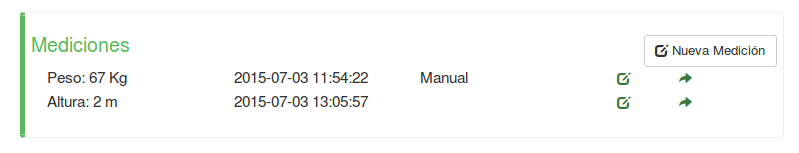
\includegraphics[width=1\textwidth]{img/2-prueba_2}
        \caption{perfil de medicion de usuario con id:3}
		\label{perfil_id_3}
\end{figure}


%\end{minipage}
    }
\clearpage

%%%%%%%%%%%%%%%%%%%%%%%%%%%%%%%%%%%%%%%%%%%%%%%%%%%%%%%%%

{\scriptsize
	\begin{table}[h]
	\centering
	\begin{tabular}{||l|p{10cm}||}
    	\rowcolor[gray]{0.9}
	    \hline 
        \hline 
	    \textbf{Caso de prueba} & \textbf{Editar Medición}\\  \hline
	    \textbf{Descripción del escenario}&  Nombre: Marita; Apellido Martinez; fecha de Nacimiento:20-08-1989; id:3; id:3; Peso 1: 67kg, id:17; peso 2: 55kg, id:16\\ \hline
	    \textbf{Criterio de aceptación}& \textbf{Cuando el usuario seleccione una medición  y luego quiera editarla. El sistema le permitirá la correspondiente edición}\\ \hline
        \textbf{Datos de entrada}& peso:65Kg \\ \hline
        \textbf{Condiciones de  prueba}& Usuario logueado con al menos una medida cargada \\ \hline \hline
	    \end{tabular}
	    \end{table}
	}
    

	\begin{longtable}{|p{5cm}|p{5cm}|p{4cm}|}
	    \hline \hline \rowcolor[gray]{0.9}
        \multicolumn{3}{||l|}{\textbf{Procedimiento de Prueba - Editar mediciones}} \\ \hline
	    \hline 
        \rowcolor[gray]{0.9}
	    \textbf{Actor} & \textbf{Sistema}& \textbf{Resultado Esperado} \\  \hline
	    El usuario, ya logueado selecciona el botón de editar de una de las mediciones (medición peso 67Kg) que se muestra en su perfil de mediciones& & \\ \hline
        & El sistema valida las que las cookies estén activas & \\ \hline
        & El sistema consulta a la API la medición 17 correspondiente al perfil con id:3 & Se muestra el perfil del formulario de carga de mediciones. con los datos precargados de la medición seleccionada\\ \hline        
	    El usuario modifica los datos de la medición seleccionada cambiando 67 por 65&  &\\ \hline
        & el sistema confirma la carga guardando los datos en la API a través del método PUT&\\ \hline
        &El sistema redirecciona al usuario a la vista de perfil de mediciones&  Se le presenta al usuario la vista de las ultimas mediciones realizadas. Mostrando 65Kg \\ \hline
        		\caption{Procedimiento de prueba para criterio de aceptación 3}
	    \end{longtable}
	
            {\scriptsize
	\begin{table}[h]
	\centering
	\begin{tabular}{|l|p{10cm}|}
	    \hline 
	    \textbf{Salida obtenida}& La vista presento la medición modificada de forma correcta\\ \hline
	    \textbf{Resultado}& \textbf{Correcto}\\ \hline
        \textbf{¿Qué fue mal?}& Nada\\ \hline      
        \textbf{Evidencia}&  En la figura \ref{edicion_medicion} se puede ver como el formulario se encuentra precargado con los valores de la medición que se desea editar, en el Json \ref{JsonMedicionModificada} se puede observar que se modifico el valor del peso y que ha cambiado la fecha de carga \\ \hline
        \textbf{Seguimiento}& No es necesario ya que el caso de prueba no causó
fallos\\ \hline
        \textbf{Estado}& \textbf{Terminado}\\ \hline        
        \textbf{¿Qué se puede mejorar?}& En otro sprint se debería añadir carteles de avisos, informando que la edición fue realizada con éxito \\ \hline              
	    \end{tabular}
        \caption{Resultado esperado para el criterio de aceptación 3}
    	\end{table}
	}
\begin{figure}[h]
        \centering
        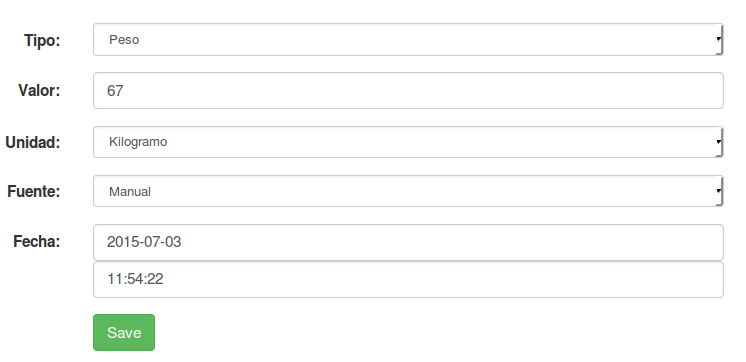
\includegraphics[width=1\textwidth]{img/2-prueba_3}
        \caption{Formulario de edición de medición}
		\label{edicion_medicion}
\end{figure}

\begin{lstlisting}[language=json,firstnumber=1,  breaklines=true, caption= Json de las medicion modificada del perfil id:3, label=JsonMedicionModificada]
{
	"id": 17,
    "measurement_source": 
	{
    	"id": 1,
	    "description": null,
	    "name": "Manual"
	},
	"measurement_unit": 
	{
    "id": 1,
    "suffix": true,
    "symbol": "Kg",
    "name": "Kilogramo"
	},
	"measurement_type": 
    {
        "id": 1,
        "description": "Peso corporal de la persona.",
        "name": "Peso"
    },
    "value": 65,
    "datetime": "2015-07-03T11:54:22.806000"
}
\end{lstlisting}
\clearpage  

%%%%%%%%%%%%%%%%%%%%%%%%%%%%%%%%%%%%%%%%%%%%%%%%%%%%%%%%%
		{\scriptsize
    \begin{table} [h]
    \centering
	\begin{tabular}{||l|p{10cm}||}
    	\rowcolor[gray]{0.9}
	    \hline 
        \hline 
		\textbf{Caso de prueba} & \textbf{Ingresar a mediciones} \\  \hline
	    \textbf{Descripción del escenario}& Nombre: Marita; Apellido Martinez; fecha de Nacimiento:2015-06-01; género: femenino; id:3; Peso 1: 54kg; peso 2: 55kg\\ \hline
	    \textbf{Criterio de aceptación}&\textbf{Si el usuario existe y no está logueado y quiere ingresar a ver sus mediciones. El sistema no le permitirá ingresar}\\ \hline
        \textbf{Datos de entrada}&  \\ \hline
        \textbf{Condiciones de  prueba}& El usuario no debe encontrase logueado.\\ \hline \hline
	    \end{tabular}
        \caption{Caso de prueba para criterio de aceptación 4}
    	\end{table}
		}
	

	\begin{longtable}{|p{5cm}|p{5cm}|p{5cm}|}
	    \hline \rowcolor[gray]{0.9}
        \multicolumn{3}{|l|}{\textbf{Procedimiento de Prueba -Ingresar mediciones}} \\ \hline
	    \textbf{Actor} & \textbf{Sistema}&\textbf{Resultado Esperado} \\  \hline
	   El usuario selecciona la pestaña de mediciones, para ver sus mediciones & & \\ \hline
        & El sistema  verifica que exista una cookies activa como na existe no lo redirección a ninguna parte &  Se muestra la ventana de logueo \\ \hline
   \caption{Procedimiento de prueba para criterio de aceptación 4}        
    \end{longtable}
 


{\scriptsize
	\begin{table}[h]

	\centering
	\begin{tabular}{|l|p{10cm}|}
	    \hline 
	    \textbf{Salida obtenida}&Se obtuvo lo q se esperaba, ya que no fue enviado a la vista de mediciones.\\ \hline
	    \textbf{Resultado}& \textbf{Correcto}\\ \hline
        \textbf{¿Qué fue mal?}& Nada\\ \hline        
        \textbf{Evidencia}&No es necesaria  \\ \hline
        \textbf{¿Qué fue mal?}& Nada\\ \hline      
        \textbf{Seguimiento}& No es necesario ya que el caso de prueba no causó fallos \\ \hline
        \textbf{Estado}& \textbf{Terminado}\\ \hline        
        \textbf{¿Qué se puede mejorar?}& En una futura iteración se podría añadir carteles de avisos informando de la situación\\ \hline              
	    \end{tabular}
        \caption{Resultado esperado para el criterio de aceptación 4}
   	\end{table}
	}

%%%%%%%%%%%%%%%%%%%%%%%%%%%%%%%%%%%%%%%%%%%%%%%%%%%%%%%%%%%%%%%%%%

\clearpage
\subsubsection{Pruebas de integración entre módulos del Sistema}
Estas pruebas se realizarán mas adelantes
\subsubsection{Pruebas de carga}
En este sprint no se realizarán este tipo de pruebas.
\subsubsection{Pruebas de seguridad por niveles de usuario}
En este sprint no se realizarán este tipo de pruebas, ya que la seguridad será un tema a tratar más adelante.

\subsection{Pruebas ejecutadas}
Aquí se realizará una conclusión general de lo que se descubrió en las pruebas.
        %
	\begin{itemize}
		\item \textbf{¿Qué fue bien?}
        	\begin{itemize}
				\item        Las cargas y ediciones se llevan a cabo correctamente.
			\end{itemize}

   		\item \textbf{¿Qué se mejoró?}
        	\begin{itemize}
				\item \textbf{Cerrado} Al crear una nueva medición, se mostraba un cartel (alert de javascript) con una fecha, dicho alert fue eliminado.
                \item \textbf{Cerrado} Se encontró un problema con la zona horaria que usa el servidor y la zona horaria del usuario, para solucionarlo hubo q hacer un casteo previo cuando se solicitaba la fecha y hora del usuario para mostrar.
			\end{itemize}

   		\item \textbf{¿Qué se puede mejorar?}
        	\begin{itemize}
		        \item \textbf{Abierto} En el futuro se deberá mejorar las validaciones de los datos a la hora de cargar información en los formularios.
        		\item \textbf{Abierto} Se deberá mejorar la manera de seleccionar la fecha y la hora.
		        \item \textbf{Abierto} Solo debería mostrarse las unidades relacionadas al tipo de medición que se ha seleccionado  
                \item \textbf{Abierto} Deberá realizarse los carteles de advertencia necesarios.
            \end{itemize}
        

	\end{itemize}